\documentclass{article}
\usepackage{hyperref}
\usepackage{amscd,amsmath,amsthm,amssymb}
\usepackage{enumerate,varioref}
\usepackage{epsfig}
\usepackage{graphicx}
\usepackage{mathtools}
\usepackage{tikz}
\usepackage{pgfplots}
\newtheorem{thm}{Theorem}
\newtheorem{cor}[thm]{Corollary}
\newtheorem{lem}[thm]{Lemma}
\newtheorem{prop}[thm]{Proposition}
\theoremstyle{definition}
\newtheorem{defn}[thm]{Definition}
\theoremstyle{remark}
\newtheorem{ex}[thm]{Example}
\newtheorem{rem}[thm]{Remark}
\numberwithin{equation}{section}
\DeclareMathOperator\arcosh{arcosh}
\newcommand{\R}{\mathbb{R}}
\newcommand{\Z}{\mathbb{Z}}
\newcommand{\C}{\mathbb{C}}
\newcommand{\Q}{\mathbb{Q}}
\newcommand{\half}{\frac{1}{2}}


\title{A Random Walk Through North America}
\author{Clark Alexander, Ivonne Garcia, Abdul Alanazi,\\
Ross Nelson, Vincent Chan}


\begin{document}
\maketitle

\begin{abstract}
We build a discrete graph of the contiguous states of The United States, Mexico, and Canada including Washington, D.C. and The Federal District of Mexico City.  From this graph we determine its chromatic number and consider two types of random walks on the graph.  The First is the classical random walk where we show that the walk converges to a stable vector in time $O(\lambda_2^t)$ where $\lambda_2$ is the second largest eigenvalue of the walking matrix.  Second, we consider a continuous time quantum walk on North America and show that the walk does not converge, but that we can increase hitting time.
\end{abstract}


\section{Introduction}

This project grew out of several ideas bandied about in a group of undergraduate math and computer science classes, and a desire to compute a nontrivial example.  Originally we were talking about Eulerian and Hamiltonian circuits on connected graphs and showing that these cannot exist on the stand alone graph of the United States or Mexico since they each have vertices of degree one (Maine and Baja California Sur respectively).  Additionally, we discovered that a large amount of the Western United States is three-colorable, and so we set out to find the obstructions to three-colorability in the entire graph.  Interestingly,but perhaps not surprisingly the addition of Canada breaks the three-colorability of the Western United States.  Additionally, the addition of Mexico to the southern border of the United States prevents the graph from having chromatic number 3.  We also know that all planar graphs have chromatic number less or equal to 4, so we set out to present a visually pleasing planar four-colored graph of North America.  In section 2, we present our graph with and without chromaticity.  In a class on quantum algorithms we were discussing discrete time quantum walks and realized that continuous time quantum walks are somewhat easier to compute.  Thus we set up the rest of our paper as such: in section 3 we present some of the early notions of classical random walks on graph, including convergence in undirected graphs to a stable vector, hitting and mixing time. In section 4 we present some of these calculations.  In section 5 we present the difference between classical and continuous quantum walks and show that the quantum walk does not converge.  Finally in the appendix we present our open source code for computing random walks and continuous time quantum walks in octave.  The graph and the code will be freely available on github at (give address, probably put this in the references) 


\section{The Graph of North America}

include graphs, scale them, explain what's going on.  Show the coloration. 



\section{The Chromatic Number of North America}

State the four-color theorem, give a reference.  Use Ross's proof that this graph has chromatic number $>3$.  There are a couple of other instances, for example and vertex 74, there is a very clear copy of $K_4$.  See if we can find a couple more. 



\section{Generalities on Classical Random Walks}

%This will mostly be my (Clark's section) I'll talk about constructing the matrices, how walks work, spectral gaps, hitting, mixing, covering, etc.  Maybe I'll mention directed walks?  Is that of any interest to any of you?

To begin our discussion of classical random walks on graphs let's begin with the easy example of walking along a line.  Suppose we have a graph of vertices labeled $\{-n,-n+1,\dots,-1,0,1,\dots,n-1,n\}$.  Our random walker will begin at the vertex labeled zero and flip a coin.  If this coin lands on ``heads" then the walker moves to vertex 1, if ``tails" then the walker moves to vertex -1.  Continuing the process at any given vertex, the walker will flip a coin and ``heads" mean the walker will move from $v$ to $v+1$.  If the coin lands ``tails" then the walker moves from $v$ to $v-1$. After some number of coin flips we see where the walker is standing.  This process gives us a probability distribution identical to the balanced binomial distribution.  
\begin{center} 
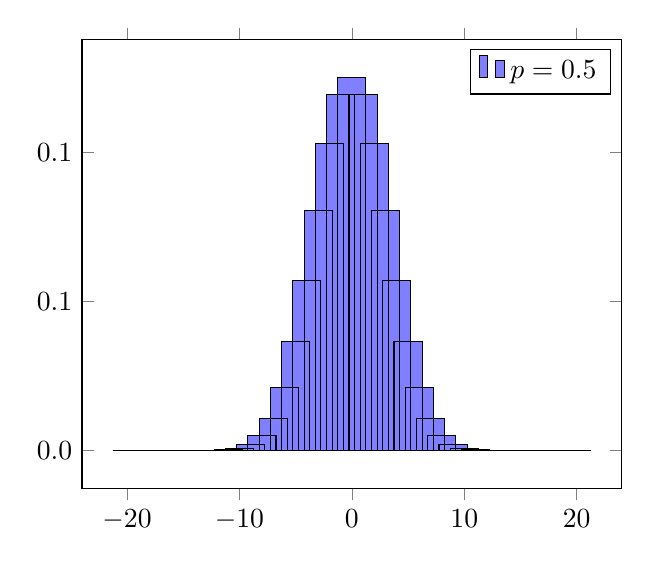
\begin{tikzpicture}[
    declare function={binom(\k,\n,\p)=\n!/((\k+20)!*(\n-(\k+20))!)*\p^(\k+20)*(1-\p)^(\n-(\k+20));}
]
\begin{axis}[
    samples at={-20,...,20},
    yticklabel style={
        /pgf/number format/fixed,
        /pgf/number format/fixed zerofill,
        /pgf/number format/precision=1
        },ybar=0pt, bar width =2.5
    ]
\addplot [fill=blue, fill opacity=0.5] {binom(x,40,0.5)}; \addlegendentry{$p=0.5$}
\end{axis}
\end{tikzpicture}
\end{center}
 
In order to formalize this we consider a general (undirected) graph $G$ with vertex set $V$ and edge set $E$.  We need not require the graph to be connected, but in all the examples that follow, we will only discuss the case of connected graphs.  Consider the walking matrix $W$ which we define by
\begin{equation}
W_{i,j} = \left\{ \begin{array}{c l}
1/deg(v_i) & \textrm{ if } (v_i,v_j)\in E\\ 
0 & \textrm{ else }
\end{array}
\right.
\end{equation}

Consider then our graph from above with 7 vertices 
\[
V = \{-3,-2,-1,0,1,2,3\}
\] and 6 edges 
\[
E = \{(-3,-2),(-2,-1),\dots,(2,3) \}
\]

\[
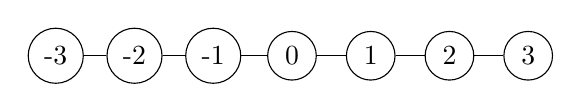
\begin{tikzpicture}
\node[circle,draw](-3) at (0,0){-3};
\node[circle,draw](-2) at (1,0){-2};
\node[circle,draw](-1) at (2,0){-1};
\node[circle,draw](0) at (3,0){0};
\node[circle,draw](1) at (4,0){1};
\node[circle,draw](2) at (5,0){2};
\node[circle,draw](3) at (6,0){3};
\foreach \from/\to in {-3/-2,-2/-1,-1/0,0/1,1/2,2/3}
 \draw (\from) -- (\to);
\end{tikzpicture}
\]


We have the following relevant matrices
\begin{eqnarray}
A & = & \begin{bmatrix}
0 & 1 & 0 & 0 & 0 & 0 & 0\\
1 & 0 & 1 & 0 & 0 & 0 & 0\\
0 & 1 & 0 & 1& 0 & 0 & 0\\
0 & 0 & 1 & 0 & 1 & 0 & 0\\
0 & 0 & 0 & 1 & 0 & 1 & 0\\
0 & 0 & 0 & 0 & 1 & 0 & 1\\
0 & 0 & 0 & 0 & 0 & 1 & 0\\
\end{bmatrix}\\
D & = & \begin{bmatrix}
1 & 0 & 0 & 0 & 0 & 0 & 0\\
0 & 2 & 0 & 0 & 0 & 0 & 0\\
0 & 0 & 2 & 0 & 0 & 0 & 0\\
0 & 0 & 0 & 2 & 0 & 0 & 0\\
0 & 0 & 0 & 0 & 2 & 0 & 0\\
0 & 0 & 0 & 0 & 0 & 2 & 0\\
0 & 0 & 0 & 0 & 0 & 0 & 1\\
\end{bmatrix} \\
W & = & \begin{bmatrix}
0 & 1 & 0 & 0 & 0 & 0 & 0\\
\half & 0 & \half & 0 & 0 & 0 & 0\\
0 & \half & 0 & \half & 0 & 0 & 0\\
0 & 0 & \half & 0 & \half & 0 & 0\\
0 & 0 & 0 & \half & 0 & \half & 0\\
0 & 0 & 0 & 0 & \half & 0 & \half \\
0 & 0 & 0 & 0 & 0 & 1 & 0\\
\end{bmatrix}\\
L & = & \begin{bmatrix}
1 & -1 & 0 & 0 & 0 & 0 & 0\\
-1 & 2 & -1 & 0 & 0 & 0 & 0\\
0 & -1 & 2 & -1 & 0 & 0 & 0\\
0 & 0 & -1 & 2 & -1 & 0 & 0\\
0 & 0 & 0 & -1 & 2 & -1 & 0\\
0 & 0 & 0 & 0 & -1 & 2 & -1\\
0 & 0 & 0 & 0 & 0 & -1 & 1\\
\end{bmatrix}
\end{eqnarray}

These are the adjacency matrix $A$, the degree matrix $D$, the stochastic walking matrix $W = AD^{-1}$, and the Laplacian matrix $L = D-A$.

Since $W$ is a stochastic matrix is takes probability distributions to probability distributions.  Then we define the probability distribution of a random walk starting at vertex $v$ and walking for $k$ steps by
\begin{equation}
p^{(k)}(v) = (v W^k)
\end{equation}

In particular the probability of finding the walker starting from vertex $i$ and walking $k$ steps at vertex $j$ is $p^{(k)}_{i,j}$.


Notice that while we tend to use column vectors in linear algebra class, we use row vectors to perform our random walk.  We reason through this on graphs which are not regular as we check all the adjacencies first and then apply the probabilities.  Equivalently we could consider the random walk $p^{(k)} = (W^t)^k v^t$.


\subsection{Other Notions of Random Walks on Graphs}

Given a graph $G$ with relevant matrices $A,D,W,L$ we define the following notions.

\begin{defn}
The \emph{hitting time} $H(i,j)$ from vertex $i$ to vertex $j$ is the expectation of the number of steps to the first time a random walker is at vertex $j$ starting at vertex $i$.
\end{defn}

\begin{defn}
The \emph{commute time} $\kappa(i,j)$ is the expectation time for a random to return to vertex $i$ after having reached vertex $j$.
\[
\kappa(i,j) = H(i,j) + H(j,i)
\]
\end{defn}

\begin{defn}
The \emph{cover time} from vertex $v$ is the expected time it takes to reach every vertex in the graph. 
\end{defn}

In a regular graph this is a constant for any given vertex.  If the graph is not regular and no particular vertex $v$ is given the cover time is the maximum amongst all vertices in the graph.

\begin{defn}
The \emph{mixing rate} is how fast a walk converges to a stationary distribution.  For a connected graph the stationary distribution $\pi$ is given by
\begin{equation}
\pi(j) = \frac{deg(j)}{2|E|}
\end{equation}
and the mixing rate is defined by
\begin{equation}
\mu = \limsup_{k\rightarrow \infty} \max_{i,j} \left| p_{ij}^{(k)} - \pi(j) \right|
\end{equation}
\end{defn}

There are several important ideas to consider with the above definitions.  First, hitting time is not symmetric.  Consider the lollipop graph
\[
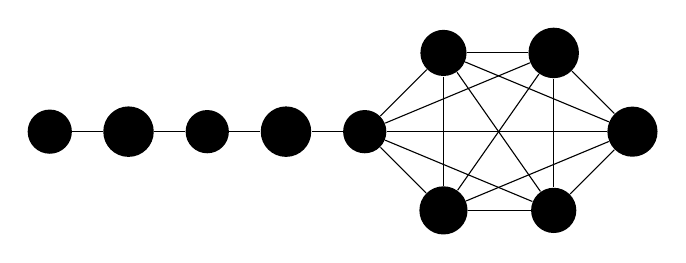
\begin{tikzpicture}
\node[circle, fill](a) at (0,0){a}; 
\node[circle, fill](b) at (1,0){b};
\node[circle, fill](c) at (2,0){c}; 
\node[circle, fill](d) at (3,0){d};
\node[circle, fill](e) at (4,0){e}; 
\node[circle, fill](f) at (5,1){f};
\node[circle, fill](g) at (5,-1){g}; 
\node[circle, fill](h) at (6.4,1){h};
\node[circle, fill](i) at (6.4,-1){i};
\node[circle, fill](j) at (7.4,0){j};
\foreach \from/\to in {a/b,b/c,c/d,d/e,e/f,e/g,e/h,e/i,f/g,f/h,f/i,g/h,g/i,h/i,e/j,f/j,g/j,h/j,i/j}
 \draw (\from) -- (\to);
\end{tikzpicture}
\]

with a complete graph on the right hand side and a simple 2-regular graph glued to it on the left.  The hitting time from the leftmost vertex to the rightmost vertex is significantly smaller than the hitting time from the rightmost vertex to the leftmost vertex.
\[
H(\textrm{left},\textrm{right}) =  < H(\textrm{right},\textrm{left}) =
\]

\section{The Walk Through North America}

Here we'll show our explicit computations, via Octave code.  present multiple graphs, use starting vectors in places like Missouri, Tennessee, Texas.  Linear combinations of such.  Compute the constant
$C(v_0)$ for each starting vector $v_0$ where
\[
\| v_0 W^k - \pi \| \sim C(v_0)\lambda_2^t
\]
 
where $\pi$ is the stable vector in this case.  We'll do this for the lazy walk and the parametrized lazy walk.  Let's also consider probabilities of starting in USA by population, Mexico by population, Canada by population, and also in the entirety of North America by population.  What is the smallest possible $C$? given that we do not start at the stable vector?  What is the difference in the values of $C(v_0)$ for the standard walks and what about $C$ for the parametrized lazy walk with matrix
\[
\alpha I + (1-\alpha)W
\]  
Generally $\alpha = \frac{1}{2}$ for the lazy walk, but I don't see any reason why we need exactly $\frac{1}{2}$.  Let's play around with this.  We can automate some code that will pick this info. 
 

\section{A Quantum Mechanical Extension}

This again is my (Clark's) section.  I'll 
explain how continuous time quantum walks work, and then we'll compute some.  We'll show that this walk does not converge to the stable vector.  The easiest way to do this is to use $\pi$ as our starting and stopping vector and show that the probability is significantly smaller than 1 for all times $t>0$.

\section*{Appendix: Code in Octave}

Present the code in octave

\begin{thebibliography}{99}
\bibitem{Random Walks} Add some things here
\bibitem{Git} github page with codes.
\end{thebibliography}






\end{document}